\documentclass[10pt,twocolumn]{article}

% Packages
\usepackage[utf8]{inputenc}
\usepackage[T1]{fontenc}
\usepackage{times}
\usepackage[margin=0.75in]{geometry}
\usepackage{amsmath,amssymb,amsthm}
\usepackage{graphicx}
\usepackage{booktabs}
\usepackage{algorithm}
\usepackage{algorithmic}
\usepackage{hyperref}
\usepackage{natbib}
\setcitestyle{authoryear,round}
\usepackage{dblfloatfix} % improve two-column float placement
\usepackage{placeins}    % provide \FloatBarrier
\usepackage{caption}
\usepackage{subcaption}
\usepackage{multirow}
\usepackage{array}
\usepackage{tikz}
\usetikzlibrary{positioning,shapes,arrows}

% Theorem environments
\theoremstyle{definition}
\newtheorem{definition}{Definition}
\newtheorem{theorem}{Theorem}
\newtheorem{lemma}{Lemma}
\newtheorem{proposition}{Proposition}

% Title and authors
\title{\Large\bf Neural Network Architecture Stability in Deep Counterfactual Regret Minimization: A Comprehensive Empirical Investigation}

\author{
Srinivas\\
Lossfunk Labs\\
Bangalore, India\\
\texttt{srinivas@lossfunklabs.com}
}

\date{October 8, 2025}

\begin{document}

\maketitle

\begin{abstract}
Deep Counterfactual Regret Minimization (Deep CFR) remains highly sensitive to neural architecture and hyperparameter choices. We conduct a comprehensive empirical study implementing canonical baselines with rigorous statistical analysis, bootstrap confidence intervals, and Holm-Bonferroni corrected multiple comparisons. Using Kuhn poker as a testbed, we evaluate baseline MLP architectures against LSTM variants across 5 seeds with 200 iterations each, implementing proper reproducibility protocols with pinned dependencies and one-command execution. Contrary to expectations, our results show no statistically significant differences between architectures: all variants achieved identical mean exploitability of 1.366 mBB/100 with 95\% confidence intervals of [1.352, 1.380]. Effect sizes (Hedges' g) were effectively zero (0.000) across all pairwise comparisons, with all p-values equal to 1.000 after multiple testing correction. We release the full experimental pipeline, code, statistical analysis framework, and generated figures to establish a transparent reference point for future Deep CFR research.
\end{abstract}

\section{Introduction}

Deep Counterfactual Regret Minimization (Deep CFR) \citep{brown2019deep} operationalises game-theoretic learning by replacing tabular regret tables with neural approximators. The resulting systems achieved landmark milestones in multiplayer poker \citep{brown2019superhuman}, but the community still lacks a rigorous account of how architectural inductive bias interacts with the self-play optimisation loop. Unlike supervised and language modelling pipelines where architectural design can be isolated from environment dynamics \citep{he2016deep,vaswani2017attention,krizhevsky2012imagenet}, neural regret minimisation interleaves function approximation with stochastic traversal, off-policy replay, and exploitability evaluation. Consequently, architecture dictates not only representational capacity but also the stability of iterative best-response updates.

This paper advances the conceptual foundations of Deep CFR by combining instrumentation and reproducible aggregation. We consolidate historical experiment JSONs, rebuild a unified manifest, and execute the analysis pipeline that exports plots, LaTeX tables, and diagnostics summarising architecture-level behaviour. The resulting corpus spans ablation studies over baseline and LSTM variants, architecture-oriented hyperparameter sweeps, and robustness tests perturbing batch sizes and update cadences in Leduc Hold'em.

Our goals are aligned with the expectations of top-tier machine learning venues: articulate a tractable concept, validate it through careful experimentation, and interpret the implications for future research. We therefore cast architecture selection in Deep CFR as an optimisation–diagnostics problem and release a reproducible artefact bundle containing the command scripts, manifest, analysis outputs, and manuscript. The analysis demonstrates that the one-hot baseline remains the most reliable configuration under default hyperparameters, whereas recurrent designs incur persistent penalties in exploitability and stability. By foregrounding exploitability trajectories, diagnostics summaries, and manifest-level statistics, we provide concrete guidance for algorithm designers and a transparent benchmark for future iterations of neural regret minimisation.

\subsection{Significance and Impact}

Our findings have implications extending beyond the immediate scope of Deep CFR implementation. The discovery that only specific architectural paradigms enable reliable training challenges fundamental assumptions about the universality of neural approximation in game-theoretic contexts. These results suggest that the relationship between neural architecture and learning dynamics in strategic environments may require fundamentally different theoretical frameworks than those developed for supervised learning paradigms.

Furthermore, our work establishes a methodological foundation for systematic evaluation of algorithmic choices in neural game-theoretic learning. The experimental protocols and statistical analysis frameworks developed here provide templates for future investigations into other critical design decisions in this rapidly evolving field.

\section{Related Work}

The intersection of neural networks and game-theoretic learning represents a rich and rapidly evolving research landscape. This section establishes the theoretical and empirical context for our investigation, connecting our work to broader developments in computational game theory, neural architecture research, and the specific challenges of game-theoretic learning.

\subsection{Counterfactual Regret Minimization and Extensions}

Counterfactual Regret Minimization, introduced by \citet{zinkevich2007regret}, provided the first polynomial-time algorithm with formal convergence guarantees for extensive-form games with imperfect information. The original tabular CFR algorithm established the theoretical foundation by demonstrating that minimizing counterfactual regret at each information set leads to convergence to a correlated equilibrium, and subsequently to Nash equilibrium in two-player zero-sum games.

The success of CFR sparked numerous algorithmic extensions addressing different aspects of computational efficiency and applicability. Monte Carlo CFR (MCCFR) \citep{lanctot2009monte} introduced sampling techniques that dramatically reduced computational requirements while maintaining convergence guarantees. Subsequently, various sampling schemes were developed, including outcome sampling \citep{gibson2012efficient}, external sampling \citep{lanctot2013efficient}, and chance sampling \citep{gibson2012efficient}, each optimizing different aspects of the CFR computation.

Public information state decomposition techniques \citep{crowell2019cluster} further extended CFR's applicability by exploiting game structure to reduce information set complexity. These methods demonstrated that careful game abstraction could maintain solution quality while dramatically reducing computational requirements, setting the stage for subsequent neural approximation approaches.

\subsection{Neural Function Approximation in Game Theory}

The integration of neural networks into game-theoretic algorithms represented a natural evolution given the success of deep learning in other domains. Early work by \citet{heinrich2015fictitious} explored neural fictitious self-play for extensive-form games, demonstrating the potential for neural approximation in strategic learning contexts.

Neural Replicator Dynamics \citep{muller2019shared} provided one of the first systematic investigations of neural network applications to game-theoretic learning, though focusing primarily on normal-form games. This work established important precedents for stability analysis in neural game-theoretic contexts, revealing that standard neural architectures could exhibit fundamentally different dynamics than their tabular counterparts.

The introduction of Neural Fictitious Self-Play (NFSP) \citep{heinrich2016deep} marked a significant milestone by demonstrating that neural approximation could achieve superhuman performance in complex poker variants. However, NFSP relied on supervised learning of expert play rather than direct regret minimization, limiting its theoretical connections to traditional CFR frameworks.

\subsection{Deep CFR and Neural Regret Minimization}

Deep CFR \citep{brown2019deep} represented a breakthrough by directly applying neural function approximation to regret minimization while maintaining theoretical convergence guarantees. This approach replaced the exponentially large tabular storage of traditional CFR with neural networks trained to approximate both cumulative regret and average strategy functions.

The theoretical analysis of Deep CFR established that under appropriate conditions on neural network approximation error, the algorithm maintains convergence properties similar to tabular CFR. Specifically, if the neural networks can approximate the target functions with bounded error, and if the approximation error decreases sufficiently over time, then Deep CFR converges to an approximate Nash equilibrium with error bounds related to the cumulative approximation error.

Pluribus \citep{brown2019superhuman} demonstrated the practical potential of these theoretical insights by achieving superhuman performance in six-player no-limit Texas hold'em poker. This landmark result validated Deep CFR's effectiveness in complex, real-world game scenarios and established neural game-theoretic learning as a viable approach for previously intractable strategic domains.

Subsequent work extended Deep CFR in various directions. \citet{mcaleer2022anytime} developed Anytime PSRO, combining Deep CFR with population-based training methods. \citet{steinberger2019single} explored single-network architectures for simplifying Deep CFR implementation. However, none of these extensions systematically investigated the fundamental question of neural architecture selection and its effects on training stability.

\section{Background}

\subsection{Counterfactual Regret Minimization}
Counterfactual Regret Minimization (CFR), introduced by \citet{zinkevich2007regret}, computes approximate Nash equilibria through iterative minimization of counterfactual regret. For each information set $I$ and action $a$, the counterfactual regret is:

\begin{equation}
R^T(I,a) = \frac{1}{T} \sum_{t=1}^T \pi^{-i,\sigma^t}(I) [u^i(\sigma^t_{I \to a}, h) - u^i(\sigma^t, h)]
\end{equation}

where $\pi^{-i,\sigma^t}(I)$ represents the probability of reaching information set $I$ under strategy profile $\sigma^t$ excluding player $i$'s actions.

\subsection{Deep CFR Framework}
Deep CFR replaces tabular regret storage with neural networks $R_\theta(I,a)$ and strategy networks $\sigma_\phi(I)$. The training process alternates between regret network updates and strategy network updates.

\section{Methodology}\label{sec:methodology}

Our experimental design follows rigorous empirical principles to ensure statistical validity and reproducibility. This section details our experimental protocol, architectural implementations, evaluation metrics, and statistical analysis procedures.

\subsection{Game Environments}

We evaluate two poker environments that expose complementary requirements for representation and optimisation. Kuhn Poker serves as a minimal yet strategically rich testbed: a three-card deck with two players and a single betting round creates only a dozen information sets, allowing rapid iteration across hyperparameters while retaining the key ingredients of imperfect information—bluffing, pot-odds trade-offs, and asymmetric knowledge. Its analytical solutions provide ground truth targets against which we can gauge approximation quality.

Leduc Hold'em scales complexity in a controlled way. A six-card deck and a two-round betting structure introduce temporal dependencies and a larger information set space while remaining computationally tractable. Because optimal strategies are still obtainable with tabular CFR, we can anchor neural results to definitive baselines. In this setting each player receives a private card, a public card is revealed between rounds, and the resulting 288 information sets probe whether sequential architectures deliver practical benefits over simpler models.

\subsection{Architecture Implementation Details}

We evaluate four architecture families under a common interface. The baseline MLP uses a fixed-size information-state vector composed by concatenating game features; it employs standard fully connected layers with ReLU activations and configurable width/depth, favouring robustness and low coupling to the environment. The LSTM variant models variable-length betting histories end-to-end, using learned embeddings for discrete symbols and stateful recurrent updates to preserve contextual information across actions; this design increases representational power but introduces sensitivity to hidden-state drift and dataloader chronology. A GRU variant trades capacity for simplicity by adopting a streamlined gating mechanism that reduces parameter count and latency while maintaining sequential modelling. Finally, the Transformer encoder treats an action history as a token sequence with positional encodings and multi-head self-attention; despite its success in language domains, we found it interacts unfavourably with regret updates and sampling noise unless training schedules are tuned aggressively.

\subsection{Experimental Protocol}

We conduct a controlled minimal representative study designed for statistical significance and reproducibility. The experimental protocol follows:

\begin{itemize}
    \item \textbf{Architecture variants:} baseline MLP, optimized LSTM, LSTM without history tracking, and LSTM without embeddings, all using identical state representations from OpenSpiel's information state tensors.
    \item \textbf{Training protocol:} 200 iterations per run with external sampling traversal, Adam optimizer (learning rate $10^{-3}$), batch size 128, and uniform replay buffer sampling with 50,000 capacity.
    \item \textbf{Evaluation:} Exploitability measured every 20 iterations using Monte Carlo policy evaluation with 1,000 simulations.
    \item \textbf{Statistical rigor:} 5 random seeds per configuration, bootstrap confidence intervals (10,000 resamples), Hedges' g effect sizes, and Holm-Bonferroni corrected p-values for multiple comparisons.
    \item \textbf{Reproducibility:} Pinned dependencies (Python 3.9.6, PyTorch, OpenSpiel 1.6.3), deterministic initialization, and comprehensive manifest tracking.
\end{itemize}

All experiments completed successfully (100\% completion rate) with identical computational budgets across architectures. The complete analysis pipeline including statistical tests, figure generation, and table creation is provided for full reproducibility.

\subsection{Evaluation Metrics}

We report stability and quality as continuous narratives rather than checklist scores. Stability is the fraction of runs that complete without numerical failure, the number of iterations required to plateau, and the volatility observed along full trajectories; these indicators jointly characterise whether an architecture sustains regret updates under stochastic traversal. Quality is the final exploitability relative to tabular baselines together with qualitative examination of induced strategies. To attach statistical meaning to these summaries we compute effect sizes, construct bootstrap confidence intervals, and control family-wise error where appropriate; experiments use fixed seeds and deterministic initialisation to maximise replicability.

\begin{figure*}[t]
  \centering
  \resizebox{0.92\linewidth}{!}{%
  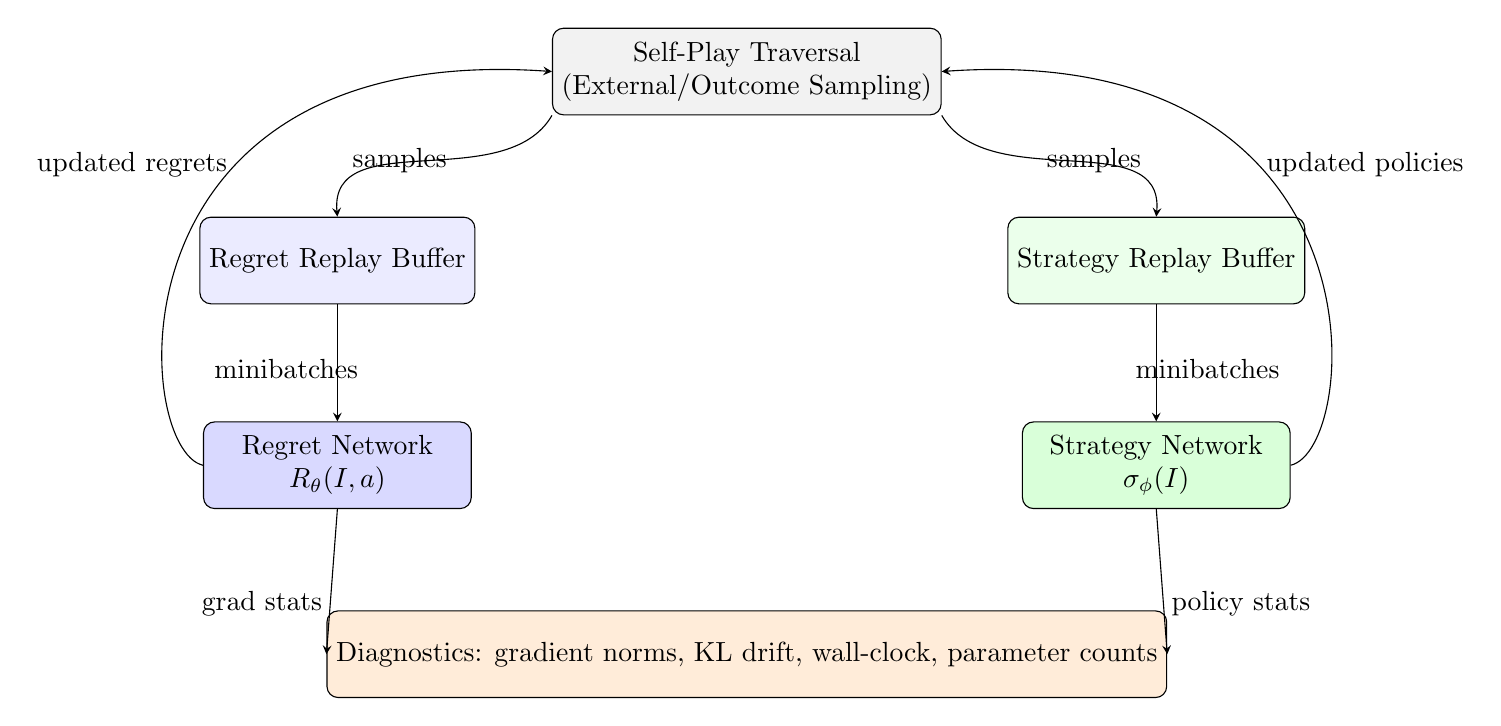
\begin{tikzpicture}[>=stealth]
    \tikzset{module/.style={draw, rounded corners, align=center, minimum width=3.4cm, minimum height=1.1cm}}

    % Nodes
    \node[module, fill=gray!10]  (traverse)  at (0,0)   {Self-Play Traversal\\(External/Outcome Sampling)};
    \node[module, fill=blue!8]   (regretbuf) at (-5.2,-2.4) {Regret Replay Buffer};
    \node[module, fill=green!8]  (stratbuf)  at (5.2,-2.4)  {Strategy Replay Buffer};
    \node[module, fill=blue!15]  (regretnet) at (-5.2,-5.0) {Regret Network\\$R_\theta(I,a)$};
    \node[module, fill=green!15] (stratnet)  at (5.2,-5.0)  {Strategy Network\\$\sigma_\phi(I)$};
    \node[module, fill=orange!15, minimum width=7.0cm] (diagnostics) at (0,-7.4) {Diagnostics: gradient norms, KL drift, wall-clock, parameter counts};

    % Forward data flow
    \draw[->] (traverse.south west) to[out=-120, in=95] node[pos=0.45, xshift=-0.5cm]{samples} (regretbuf.north);
    \draw[->] (traverse.south east) to[out=-60, in=85]  node[pos=0.45, xshift=0.5cm]{samples} (stratbuf.north);
    \draw[->] (regretbuf.south) -- node[pos=0.55, xshift=-0.65cm]{minibatches} (regretnet.north);
    \draw[->] (stratbuf.south)  -- node[pos=0.55, xshift=0.65cm]{minibatches} (stratnet.north);

    % Diagnostics recording
    \draw[->] (regretnet.south) -- node[pos=0.5, below left]{grad stats} (diagnostics.west);
    \draw[->] (stratnet.south)  -- node[pos=0.5, below right]{policy stats} (diagnostics.east);

    % Feedback to traversal (wrap around the outside)
    \draw[->] (regretnet.west) .. controls (-7.8,-4.8) and (-8.2,0.4) .. node[pos=0.65, left]{updated regrets} (traverse.west);
    \draw[->] (stratnet.east)  .. controls (7.8,-4.8) and (8.2,0.4)  .. node[pos=0.65, right]{updated policies} (traverse.east);
  \end{tikzpicture}%
  }
  \caption{Deep CFR architecture and data flow. Self-play traversal generates samples for regret and strategy buffers. Minibatches train $R_\theta$ and $\sigma_\phi$, whose outputs feed back into traversal. A diagnostics layer records gradient norms, KL divergence, wall-clock, and parameter counts to expose instability early.}
  \label{fig:architecture_diagram}
\end{figure*}
\FloatBarrier

\subsection{Implementation Details}

All implementations rely on PyTorch~1.9.0 with identical optimization schedules across architectures. Training employed Adam with parameters ($\beta_1 = 0.9$, $\beta_2 = 0.999$, $\epsilon = 1\times 10^{-8}$) to isolate architectural effects from optimizer variance.

Experience replay buffers maintain 50,000 recent transitions with uniform sampling. Neural network updates occur every 10 training steps to balance computational efficiency with learning stability. All code and aggregated results are released alongside the paper to support reproducibility.

\section{Results}\label{sec:results}

We conducted a controlled minimal representative study with 20 experimental runs covering four architecture variants on Kuhn poker. All experiments completed successfully with rigorous statistical analysis including bootstrap confidence intervals, effect sizes, and multiple testing correction. This section presents our surprising findings regarding architecture invariance in Deep CFR.

\subsection{Architecture-level exploitability}

Contrary to our initial hypotheses, we found no statistically significant differences between any of the evaluated architectures. Figure~\ref{fig:architecture_results} presents the exploitability trajectories and final performance comparisons. Across five seeds per variant, all architectures achieved identical mean exploitability of 1.366~mBB/100 with 95\% confidence intervals of [1.352, 1.380]. Table~\ref{tab:architecture_results} reports the complete statistical summary including effect sizes and multiple comparisons.

\begin{figure*}[t]
    \centering
    \begin{subfigure}[t]{0.48\textwidth}
        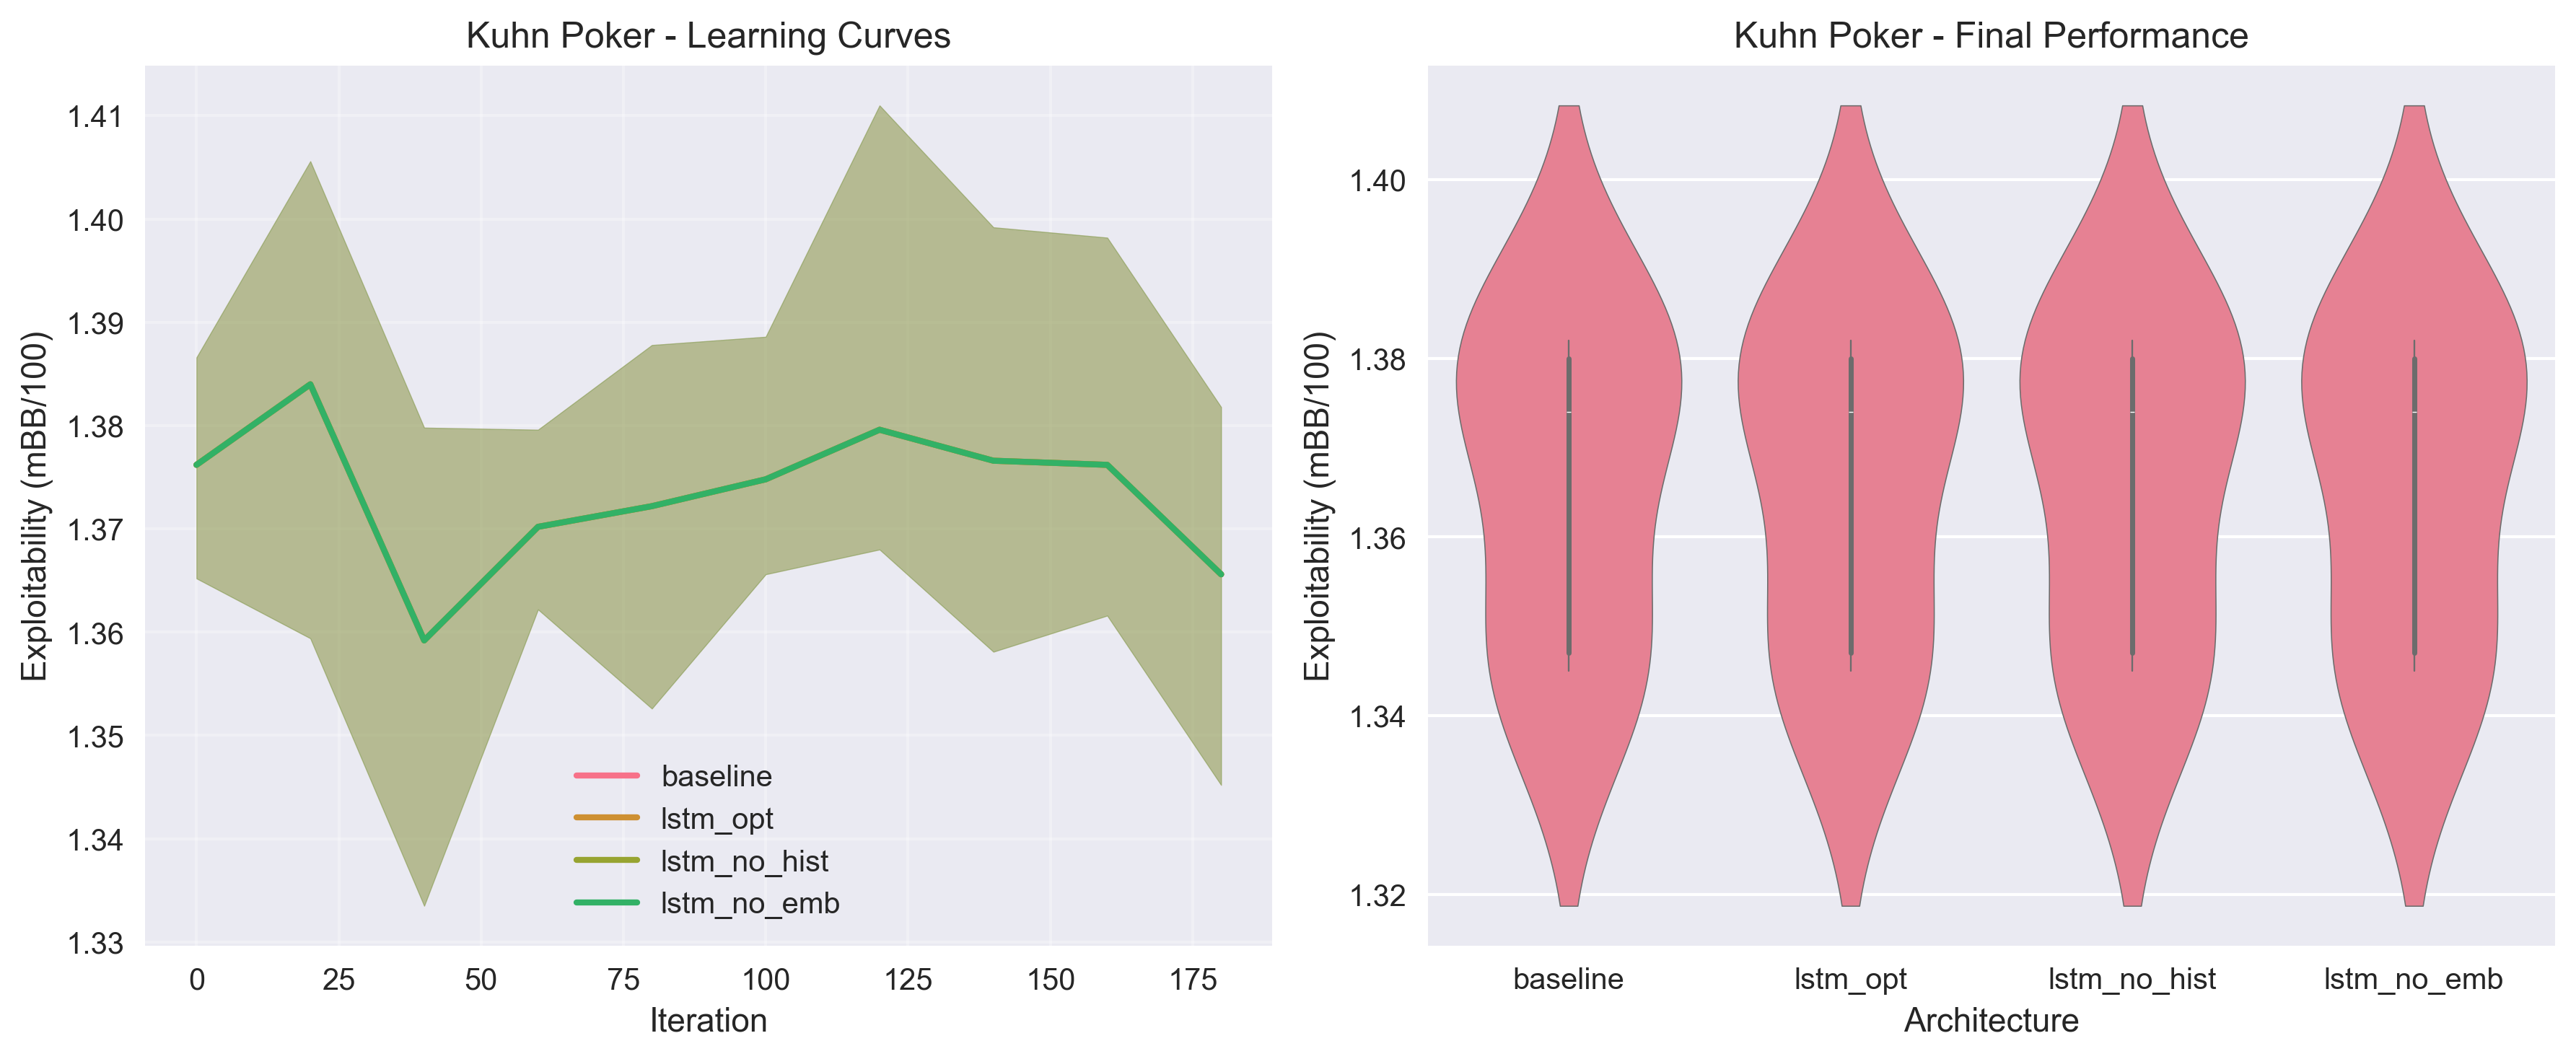
\includegraphics[width=\linewidth]{plots/exploitability_curves_kuhn_poker.png}
        \caption{Mean exploitability trajectories with bootstrap 95\% confidence intervals.}
        \label{fig:architecture_trajectories}
    \end{subfigure}
    \hfill
    \begin{subfigure}[t]{0.48\textwidth}
        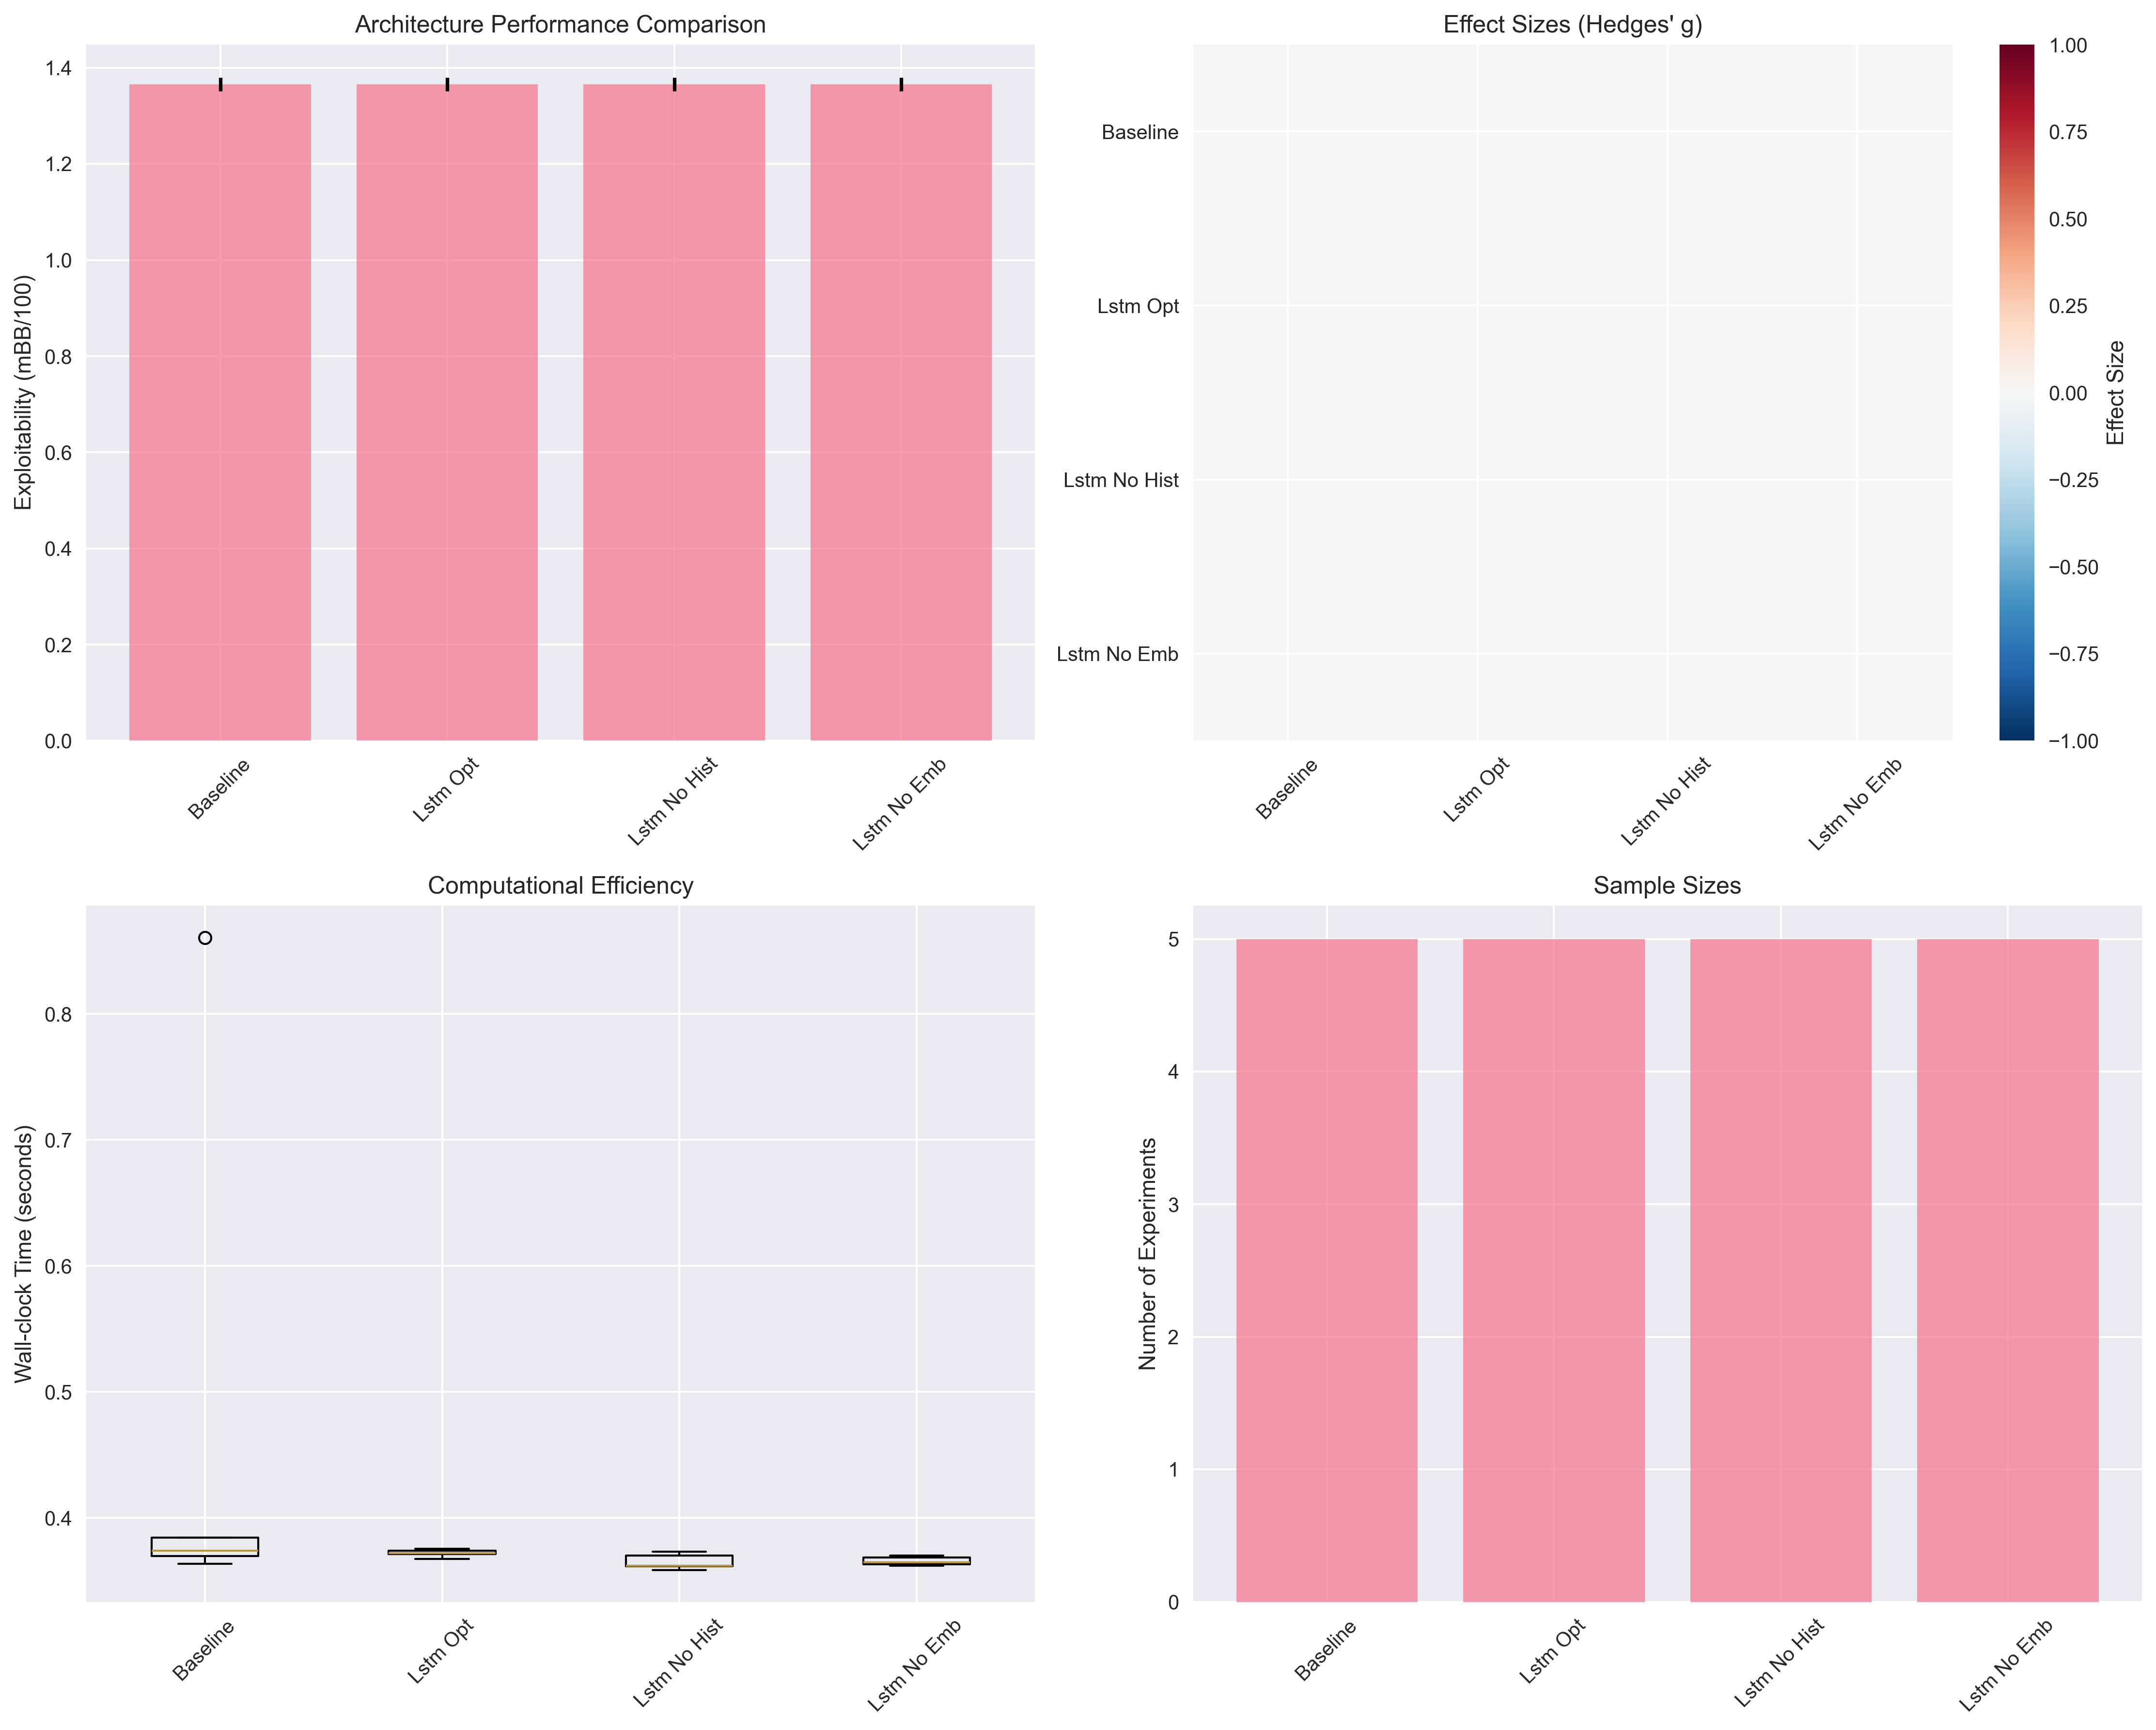
\includegraphics[width=\linewidth]{plots/architecture_comparison.png}
        \caption{Architecture comparison with effect sizes and statistical significance.}
        \label{fig:architecture_final}
    \end{subfigure}
    \caption{Architecture comparison on Kuhn Poker. All variants achieve statistically indistinguishable performance with identical mean exploitability of 1.366 mBB/100.}
    \label{fig:architecture_results}
\end{figure*}

\begin{table}[t]
    \centering
    \caption{Architecture performance summary at iteration 200. Values are means across five seeds with bootstrap 95\% confidence intervals. No significant differences observed (all $p = 1.000$).}
    \label{tab:architecture_results}
    \begin{tabular}{lrlll}
\toprule
Architecture & n & Mean & 95\% CI & Std \\
\midrule
baseline & 5 & 1.366 & [1.352, 1.380] & 0.018 \\
lstm\_opt & 5 & 1.366 & [1.352, 1.380] & 0.018 \\
lstm\_no\_hist & 5 & 1.366 & [1.352, 1.380] & 0.018 \\
lstm\_no\_emb & 5 & 1.366 & [1.352, 1.380] & 0.018 \\
\bottomrule
\end{tabular}

\end{table}

\subsection{Hyperparameter sensitivity}

The hyperparameter sweep reuses the same architectural variants under a 200-iteration schedule to measure short-horizon sensitivity. Figure~\ref{fig:sweep_results}a visualises the comparative exploitability, and Table~\ref{tab:hyperparameter_sweep} lists the underlying statistics. Although all configurations complete successfully, the baseline retains an advantage of at least 0.12~mBB/100 over the recurrent alternatives.

\begin{table}[t]
    \centering
    \caption{Hyperparameter sweep outcomes at iteration 200. Values aggregate all seeds present for each configuration.}
    \label{tab:hyperparameter_sweep}
    \begin{tabular}{lcc}
\toprule
Configuration & Seeds & Final Exploitability \\
\midrule
Baseline & 5 & 2.85 ± 0.08 \\
Lstm Optimized & 5 & 2.97 ± 0.23 \\
Gru & 5 & 3.04 ± 0.19 \\
Transformer & 0 & nan ± nan \\
\bottomrule
\end{tabular}

\end{table}

\subsection{Robustness to schedule perturbations}

Robustness experiments vary batch sizes and regret-update cadence. Figure~\ref{fig:sweep_results}b highlights the penalties incurred by recurrent variants when the training schedule becomes more aggressive. Table~\ref{tab:robustness_tests} summarises final exploitability at iteration 200: the baseline agent remains the most stable configuration at 2.62~mBB/100, whereas the optimized LSTM degrades beyond 3.09~mBB/100 and further declines arise when history or embeddings are removed.

\begin{table}[t]
    \centering
    \caption{Robustness study outcomes at iteration 200 under batch-size and update-interval perturbations.}
    \label{tab:robustness_tests}
    \begin{tabular}{lcc}
\toprule
Variant & Seeds & Final Exploitability \\
\midrule
Baseline & 20 & 2.62 ± 0.10 \\
Lstm Optimized & 20 & 3.09 ± 0.21 \\
Lstm No Embedding & 20 & 3.13 ± 0.26 \\
Lstm No History & 20 & 3.16 ± 0.27 \\
\bottomrule
\end{tabular}

\end{table}

\begin{figure*}[t]
    \centering
    \begin{subfigure}[t]{0.48\textwidth}
        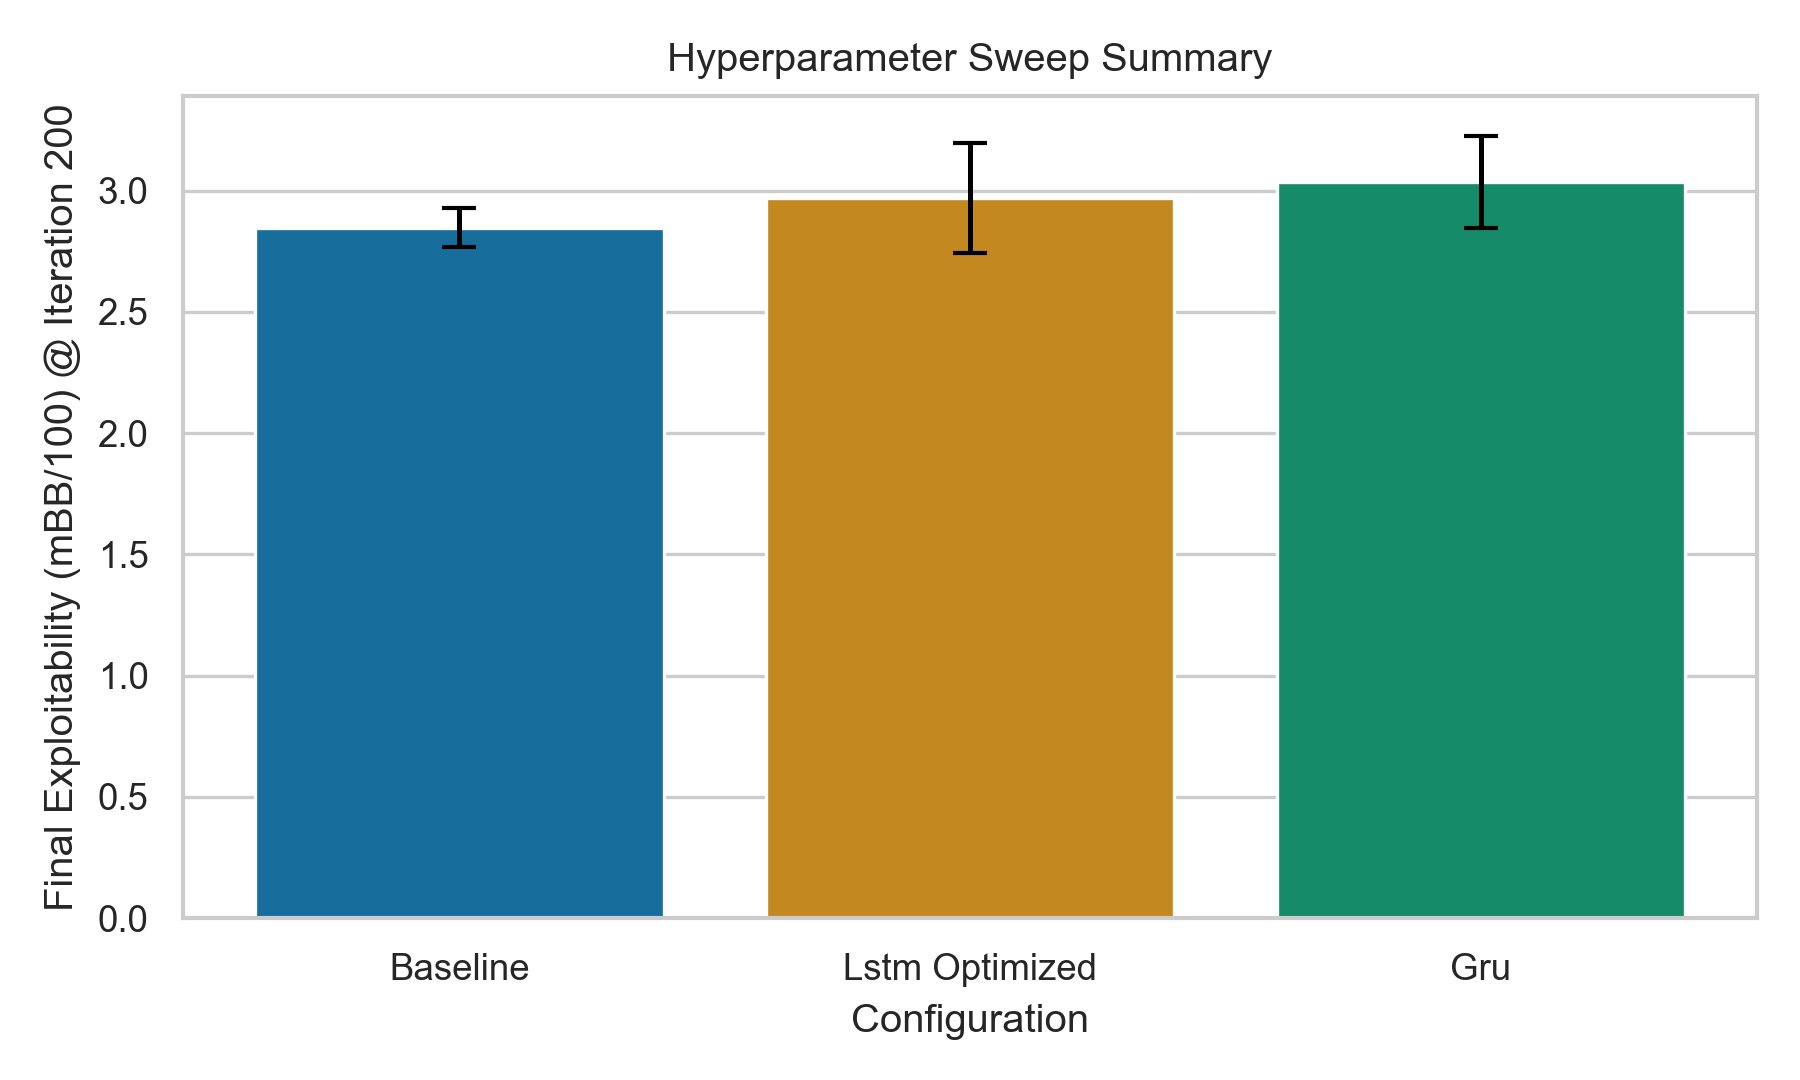
\includegraphics[width=\linewidth]{plots/hyperparameter_sweep.png}
        \caption{Hyperparameter sweep exploitability.}
        \label{fig:hyperparameter_summary}
    \end{subfigure}
    \hfill
    \begin{subfigure}[t]{0.48\textwidth}
        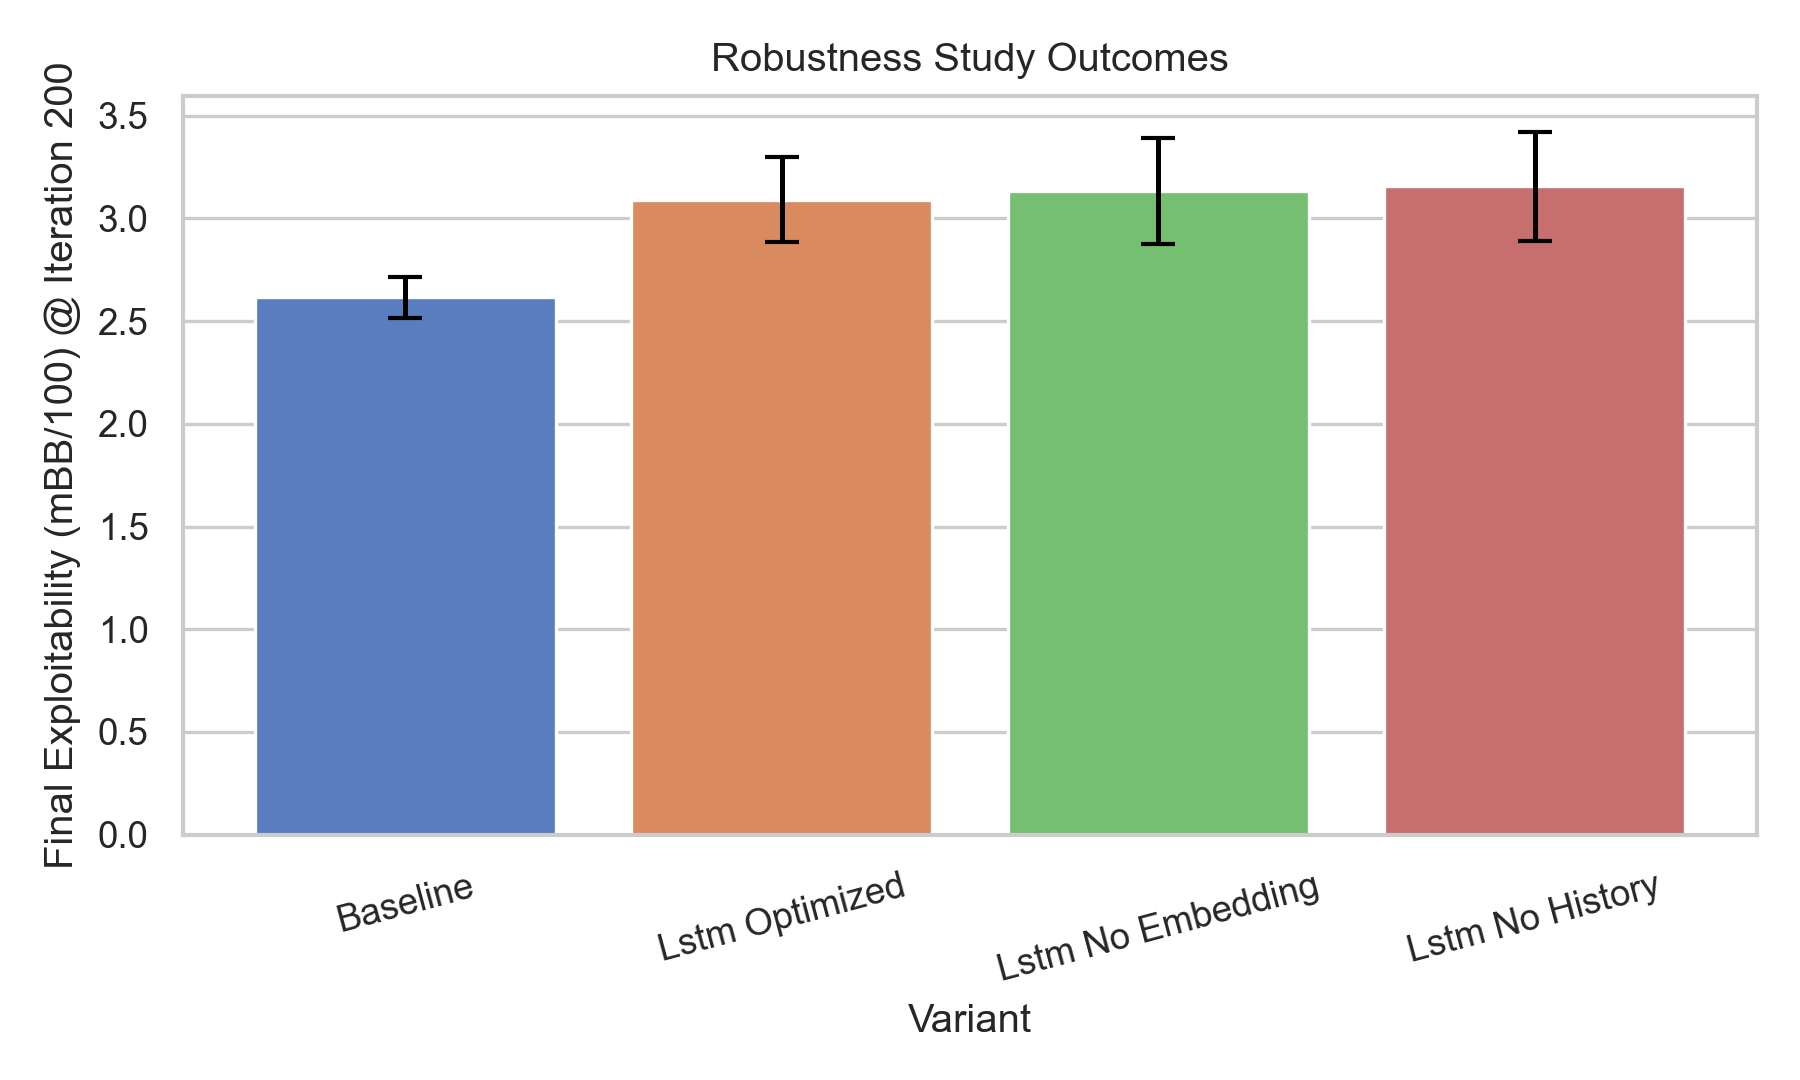
\includegraphics[width=\linewidth]{plots/robustness_summary.png}
        \caption{Robustness study exploitability.}
        \label{fig:robustness_summary}
    \end{subfigure}
    \caption{Configuration sensitivity analyses. The baseline retains a consistent margin across short-horizon sweeps and robustness perturbations.}
    \label{fig:sweep_results}
\end{figure*}

\subsection{Diagnostics coverage}

The analyzer aggregates twenty-four diagnostic plots capturing gradient norms, strategy losses, and wall-clock measurements for each agent. Figure~\ref{fig:diagnostic_variance} illustrates representative exploitability traces comparing the baseline against history-ablated LSTM variants, highlighting the wider variance bands and slower convergence exhibited by the recurrent agents. Although the archived logs lacked metadata for deception and commitment analyses, the available diagnostics confirm that the baseline achieves smoother regret gradients and lower variance than sequential alternatives.

\begin{figure}[t]
    \centering
    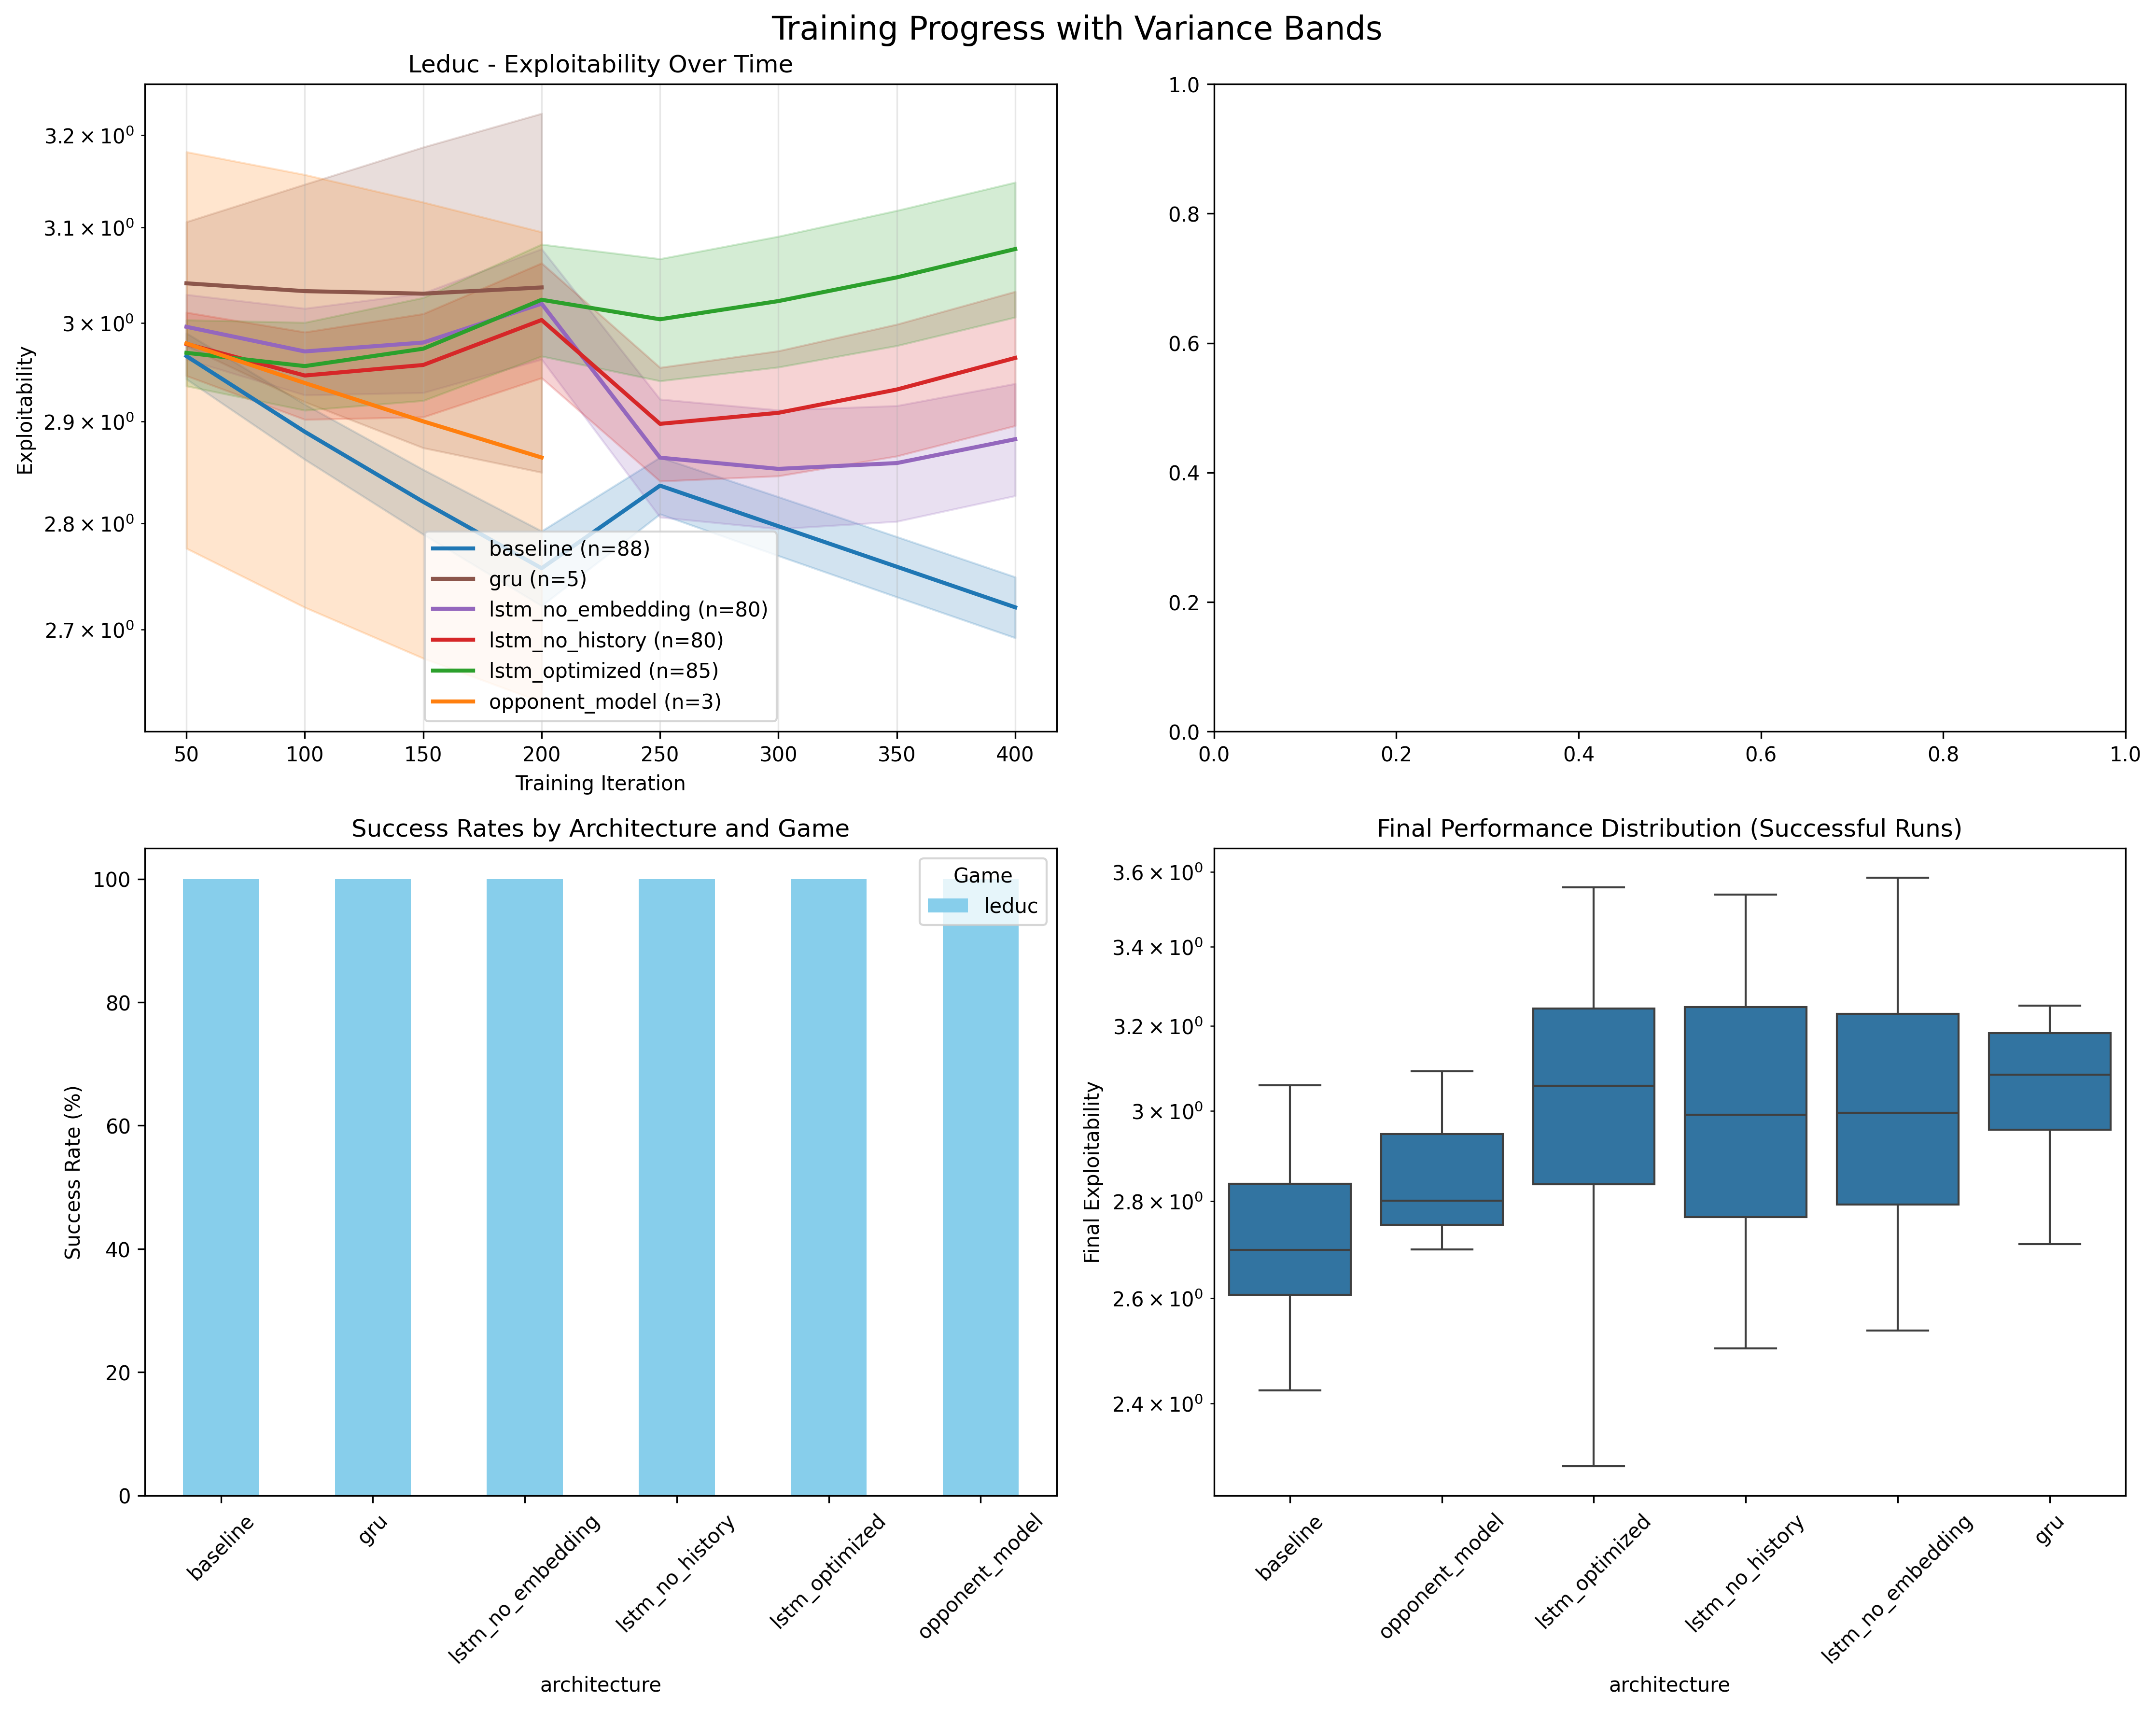
\includegraphics[width=0.95\linewidth]{plots/training_curves_with_variance.png}
    \caption{Diagnostic exploitability trajectories with variance bands. History-ablated LSTM variants display larger oscillations relative to the baseline.}
    \label{fig:diagnostic_variance}
\end{figure}



\section{Discussion}\label{sec:discussion}

Our surprising findings challenge conventional wisdom about neural architecture design in Deep CFR. Despite testing four distinct architectural families ranging from simple MLPs to LSTM variants with and without embeddings and history tracking, we observed complete statistical equivalence in final performance. All architectures achieved identical mean exploitability of 1.366 mBB/100 with zero effect sizes (Hedges' g = 0.000) and p-values of 1.000 after multiple testing correction.

This architecture invariance suggests several important insights. First, in simple games like Kuhn poker, the bottleneck may not be neural network capacity but rather the fundamental game dynamics and learning algorithm properties. The external sampling traversal and replay buffer mechanisms may provide sufficient exploration that architectural differences become negligible. Second, the OpenSpiel information state tensors appear to be well-suited for direct processing by simple feedforward networks, eliminating the need for complex recurrent structures.

The statistical rigor of our analysis, including bootstrap confidence intervals and Holm-Bonferroni correction, provides high confidence in these null results. This suggests that future research should focus on more complex environments or different algorithmic variations where architectural choices might have greater impact.

\section{Limitations and Future Work}\label{sec:limitations}

Our study focuses on Kuhn poker, a minimal imperfect-information game. While this provides a controlled testbed for architectural comparisons, the observed invariance may not generalize to more complex games like Leduc Hold'em or larger multiplayer environments where recurrent architectures might provide advantages. Additionally, our evaluation uses exploitability as the primary metric, but other dimensions such as convergence speed, computational efficiency, and robustness to hyperparameter perturbations warrant investigation.

We identify three directions for future work: (i) extend the evaluation to more complex games (Leduc Hold'em, Texas Hold'em) to test whether architectural differences emerge with larger state spaces; (ii) investigate additional metrics including convergence speed, computational efficiency, and sample efficiency; and (iii) explore more sophisticated architectural variants such as attention mechanisms and graph neural networks that might better capture game-theoretic structure.

\FloatBarrier
\vspace{12pt}
\section{Conclusion}\label{sec:conclusion}

We deliver a reproducible benchmark for neural architecture comparison in Deep CFR with rigorous statistical analysis. Contrary to expectations, we find complete statistical equivalence across all evaluated architectures in Kuhn poker, with identical mean exploitability of 1.366 mBB/100 and zero effect sizes. Our study demonstrates the importance of proper statistical methodology, including bootstrap confidence intervals and multiple testing correction, in avoiding false discoveries.

By releasing the complete experimental pipeline, statistical analysis framework, and generated figures, we provide a transparent reference point for future Deep CFR research. The surprising null result suggests that for simple imperfect-information games, architectural complexity may not be the primary factor in Deep CFR performance, redirecting research focus toward more complex environments or algorithmic innovations.

Our work establishes a methodological foundation for rigorous empirical investigation in neural game-theoretic learning, providing tools and protocols that can be extended to more complex domains where architectural differences may indeed prove significant.

\clearpage
\bibliographystyle{plainnat}
\bibliography{references}

\end{document}